% Source-page vector redraw from 2005 Spring Beijing Science, printed p. 214, Q18.
% The normalized curve and line illustrate only the source-visible topology; no parameters are inferred.
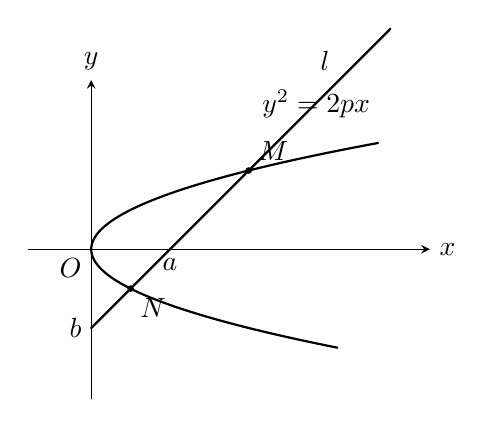
\begin{tikzpicture}[>=stealth, line cap=round, line join=round, scale=1.0]
\draw[->] (-.8,0)--(4.3,0) node[right] {$x$};
\draw[->] (0,-1.9)--(0,2.15) node[above] {$y$};
\node[below left] at (0,0) {$O$};
\draw[thick, domain=-1.25:1.35, samples=100, variable=\t]
  plot ({2*\t*\t},{\t});
% Schematic secant: it crosses y-axis below O and x-axis to the right of O.
\draw[thick] (0,-1)--(3.8,2.8);
\coordinate (M) at (2,1); \coordinate (N) at (.5,-.5);
\fill (M) circle (1.2pt) (N) circle (1.2pt);
\node[above right] at (M) {$M$}; \node[below right] at (N) {$N$};
\node[below] at (1,0) {$a$}; \node[left] at (0,-1) {$b$};
\node[above right] at (2.05,1.55) {$y^2=2px$};
\node[above left] at (3.15,2.15) {$l$};
\end{tikzpicture}
